\section{Evaluation}
\label{sec:bpm2017evaluation}

In this section, we show the applicability of our technique to project-oriented business processes and its effectiveness in uncovering work dependencies. With respect to the requirements formulated in \Cref{sec:bpm2017background}, we evaluate against requirements {R2} and {R3} in \Cref{subsec:quantitative-eval} and against requirement {R1} in \Cref{subsec:qualitative-eval}.

We implemented our techniques as a prototype\footnote{The source code is available at \url{https://github.com/s41m1r/MiningVCS}} and used it on 10 real world software projects with different sizes. The input of our program is a \gls{vcs} log and the output is a set of analysis data with information about the evolution of the artifacts and their dependencies. We report the results in \Cref{table:evaluation-results-new}. The results are listed in increasing order of project size. The parameters $\chi$ and $d$ are the metrics of \emph{degree of co-evolution} and \emph{distance}, respectively. In this example, $\chi > 0.7$ signifies that the co-evolution is high ($\chi^{H}$) and $\chi < 0.3$ that the co-evolution is low ($\chi^{L}$). As previously mentioned, this is a user customizable threshold that can be set by the domain expert. Likewise, the distance is considered low ($d^{L}$) when $d<=2$ and high ($d^{H}$) when $d>2$. The parameter  $\overline{|p_f|}$ and {$max(|p_{f}|)$} are respectively the average and the maximum lengths of the path to the root (i.e. average tree depth of the files). The column {$|A_{evo}|$} shows the average number of activities in the process representing the artifact evolution. Lastly, the columns {$\overline{d}$} and {$max(d)$} report the average and maximum file distance, respectively. Next, we use these data for a quantitative evaluation of the projects.

% Please add the following required packages to your document preamble:
% \usepackage{graphicx}
\begin{table}[t]
\centering
\caption{Evaluation of real world projects. Respectively the thresholds are: $\chi^{L}$ if $\chi < 0.3$,  $\chi^{H}$ if $\chi > 0.7$  low and high degree of co-evolution; $d^{L}$ if $d \leq 2$,  $d^{H}$ if $d > 2$ respectively low and high distance.}
\label{table:evaluation-results-new}
\resizebox{\textwidth}{!}{%
\begin{tabular}{rrrrrrrrrrrrrr}
\
Project                 & \rot{Commits} & \rot{Files} & {$\chi^{H}$} & {$\chi^{L}$} & \begin{tabular}[l]{@{}r@{}}{$(d^{L},\chi^{L})$}\end{tabular} & \begin{tabular}[l]{@{}r@{}}{$(d^{L},\chi^{H})$}\end{tabular} & \begin{tabular}[b]{@{}r@{}}{$(d^{H},\chi^{L},)$}\end{tabular} & \begin{tabular}[l]{@{}r@{}}{$(d^{H},\chi^{H})$}\end{tabular} & \rot{$\overline{|p_f|}$} & \rot{$max(|p_{f}|)$} & \rot{$|A_{evo}|$} & \rot{$\overline{d}$} & \rot{$max(d)$} \\ \midrule
%smsr                    & 21        & 6         & 22                   & 6                  & 0                          & 9                            & 6                       & 13                        & 2.71             & 5             & 1.82                    & 1.43                & 6                  \\
mwaligner  & 21      & 9     & 37                   & 7                 & 6                               & 30                                 & 1                                          & 7                                             & 1.11              & 2           & 2.40         & 0.94                 & 3                 \\
Biglist                 & 202     & 15    & 22                   & 90                & 31                              & 18                                 & 59                                         & 4                                             & 1.47              & 3            & 2.76         & 1.20                 & 5                 \\
camundaRD & 11      & 15    & 74                   & 26                & 0                               & 25                                 & 26                                         & 49                                            & 2.18              & 4            & 2.05         & 2.03                 & 7                 \\
graphql                 & 256     & 30    & 89                   & 357               & 121                             & 89                                 & 236                                        & 0                                             & 1.40              & 2            & 3.18         & 1.11                 & 4                 \\
jgitcookbook            & 135     & 89    & 773                  & 2866              & 505                             & 289                                & 2361                                       & 484                                           & 6.93              & 8            & 1.33         & 2.68                 & 14                \\
mysqlpython             & 749     & 168   & 2288                 & 11571             & 742                             & 591                                & 10829                                      & 1697                                          & 2.59              & 7            & 1.65         & 2.52                 & 11                \\
gantt                   & 23      & 228   & 7006                 & 14343             & 386                             & 3480                               & 13957                                      & 3526                                          & 3.30              & 4            & 1.71         & 2.16                 & 7                 \\
facebookjavasdk         & 38      & 293   & 16478                & 26092             & 2017                            & 16311                              & 24075                                      & 167                                           & 6.21              & 8            & 4.78         & 5.58                 & 13                \\
caret                   & 864     & 432   & 15366                & 60874             & 9538                            & 14785                              & 51336                                      & 581                                           & 3.01              & 4            & 3.15         & 1.60                 & 7                 \\
operationcode           & 1114    & 1053  & 84024                & 444605            & 2291                            & 5537                               & 442314                                     & 78487                                         & 4.27              & 8            & 2.01         & 4.85                 & 15               \\
\end{tabular}%
}
\end{table}
%\vspace*{1cm} 

%\subsection{Prototypical Implementation}
\label{subsec:prototype}


%
%The first step of the approach is the preprocess of the VCS log received as input. The main goal of this phase is generate a set of events and store them into a database. Second, we obtain different views on the stored events. In particular, we are interested in observing
%\begin{inparaenum}[\itshape i)]
%	\item all the commits that affected the files over time;
%	\item the amount of change brought by the commits to the files; and
%	\item the users who issued such commits.
%\end{inparaenum}
%The third phase is responsible for considering the different perspectives defined by the project manager and through the generated views extract the necessary knowledge. The last phase is responsible for providing the visualization combining the different perspectives considered. The following sections detail each of the phases.

We implemented our technique as a prototype\footnote{\url{https://github.com/s41m1r/MiningVCS.git}}. The input of our program is a \gls{vcs} log and the output is a set of analysis data with information about the evolution of the artifacts and their dependencies. 
%%Next we show the implementation details of \Cref{algorithm:all}.
%
%
%
%%\subsubsection{Preprocess VCS Logs.}
%As a first step (cf.~\Cref{algorithm:all}) we need to preprocess the input in order to extract events. Events in \gls{vcs} have multiple dimensions and relations among one another. Therefore, the natural way of capturing them is through a relational data model. This model serves at structuring the raw data and persisting the results after first step of \Cref{algorithm:all}. \Cref{fig:data-model} outlines the main entities in a \gls{vcs} and the relationships of our interest. The result the first step of \Cref{algorithm:all} is the correct population of the a database with the set of the extracted events, stored according to the relational schema. 
%
%\begin{figure}[]
%	\centering
%	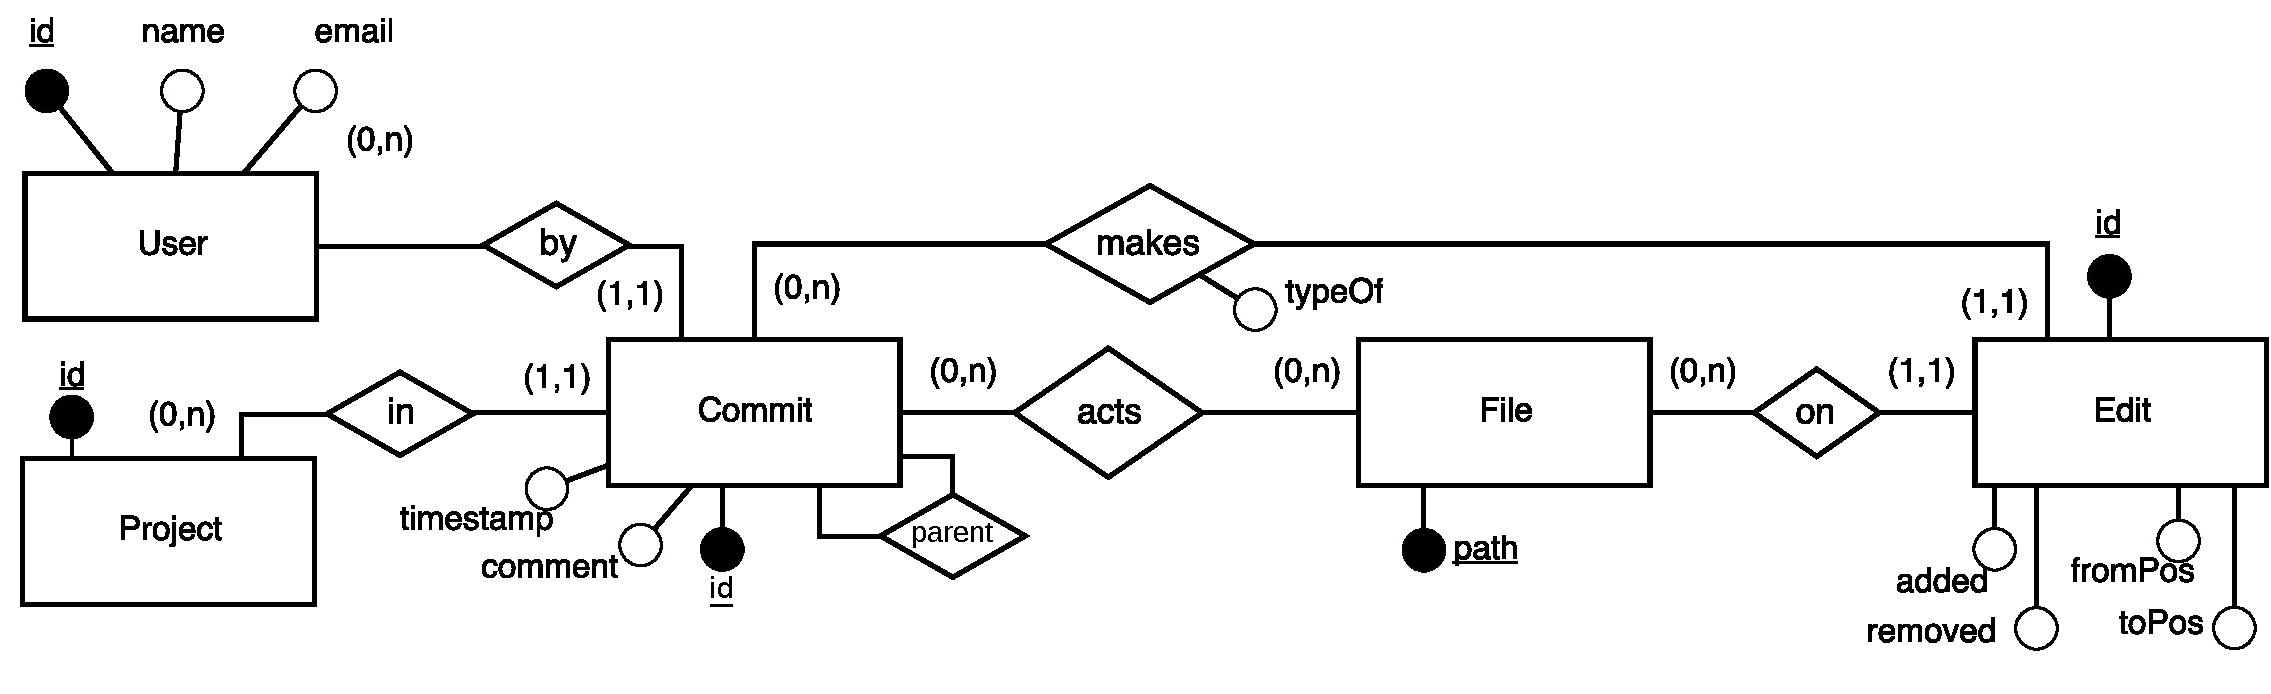
\includegraphics[width=0.9\linewidth]{figures/CommitLogER}
%	\caption{Relational schema of a software project}
%	\label{fig:data-model}
%\end{figure}
%
%%\subsubsection{Obtain View on Project.}
%
%The step~\ref{algorithm:all} makes queries over the event set in order to retrieve aggregated views from them. This is simply done by defining queries on the database and export collect their results (e.g., in a CSV file). Step~\ref{step:contaiments} consists in recreating the file structure. This is implemented by reverse engineering the directory structure from the \texttt{path} attribute of the entity \texttt{File} that is present in the output of the query. Next, we actuate step~\ref{step:evolution} by implementing \Cref{algorithm:compute-evolution} that computes the artifact evolutions. This algorithm takes as input the set of views calculated previously and outputs \begin{inparaenum}[\itshape i)]
%	\item and a set of \emph{file stories} that report the amount of change, time and comments of the file history, and
%	\item a set process that describe the evolution of every artifact obtained by story mining~\cite{Goncalves2011} the file stories.
%\end{inparaenum} Finally, for step~\ref{step:dependencies} we implement \Cref{algorithm:compute-dependencies}. This algorithm takes as input the aggregated views obtained previously and two parameters: a comparison function and a threshold. We use the Pearson correlation $\rho$ and let the domain expert set the threshold $\delta$ to filter the strength of the dependencies. An important step before 


%One example of query that outputs a view of the daily changes of the artifact \texttt{model.java} is shown in \Cref{lst:query}. 

%\begin{center}
%\begin{lstlisting}[
%language=SQL,
%showspaces=false,
%float=ht,
%xleftmargin=4em,
%aboveskip=6pt,
%belowskip=0cm,
%belowcaptionskip=0cm,
%basicstyle=\ttfamily\scriptsize,
%showstringspaces=false,
%commentstyle=\color{gray},
%mathescape=true,
%caption={SQL query to obtain the artifact history for a given artifact, aggregated on a day level},captionpos=b, label={lst:query}
%]
%SELECT CONCAT(Commit.comment,$\S$) as Comments, 
%	DATE(Commit.timeStamp) as Date, 
%	sum(linesAdded+linesRemoved) as Change, 
%	CONCAT(User.name, '$\S$') as Users
%FROM File, Edit, acts,Commit,User 
%WHERE File.path = 'model.txt' 
%	AND Edit.commit_id = Commit.id 
%	AND Edit.file_path = File.path
%	AND User.id = Commit.user_id
%	AND acts.file_path = File.path 
%	AND acts.commit_id = Commit.id
%GROUP BY Date
%ORDER By Date ASC
%\end{lstlisting}
%\end{center}
%
%\Cref{table:analysis-data} depicts a view obtained with the query in \Cref{lst:query} on the project shown in \Cref{subsec:scenario}. The data is aggregated by day. String values are concatenated together with the symbol '$\S$'.
%
%% Please add the following required packages to your document preamble:
% \usepackage{booktabs}
% \usepackage{graphicx}
\begin{table}[h]
\centering
\caption{View generated by the query in \Cref{lst:query}. Comments and users that affected the artifact at the same day are aggregated by concatenation.}
\label{table:analysis-data}
%\resizebox{\linewidth}{!}{%
\setlength{\tabcolsep}{4pt}
\begin{tabular}{@{}llllllll@{\hspace*{3pt}}}
%\toprule
Comments                                                                                                                                                                            & Date      & \rot{\#LinesAdded} & \rot{\#LinesRemoved} & \rot{TotalChange} & \rot{TotalDiff} & \rot{LinesNow} & \rot{Users}                     \\ \midrule
\rowcolor{lightgray} \begin{tabular}[c]{@{}l@{}}Modify method A to\\  meet the new requirement \\ for methods speed . \\Fix bug on  method A . \\ Create model.java . \\ Add solver methods\end{tabular} & 2017-01-31 & 36              & 1                 & 37                  & 35                & 113               & \begin{tabular}[c]{@{}l@{}}Anna  \\ John  \\ Beth  \end{tabular} \\
Implement method B                                                                                                                                                                      & 2017-02-02 & 21              & 0                 & 21                  & 21                & 56                & Anna                      \\ \rowcolor{lightgray}
Update model.java                                                                                                                                                                       & 2017-02-08 & 25              & 0                 & 25                  & 25                & 81                & Anna                      \\ \bottomrule
\end{tabular}%
%}

\end{table}

%\subsubsection{Analyze project data.}

%The input of this phase is a collection resulting from querying all the artifact histories from the data store. At this point the data is ready to be analyzed. 
%In this step analyses on the view extracted are performed. There are a number of different analyses that can be applied directly to the \emph{aggregate events}, e.g. checking whether project participants have been working on the assigned tasks ("Are they working in the artifacts they should/?") or there has rather been disorganization in regards. In this work, we focus on analyzes related to the artifacts, i.e. how they evolve over time, how they are organized and how are the dependencies among them. Therefore, in this section we focus on extracting the \emph{containments}, \emph{dependencies} and \emph{artifact evolution} elements.
%
%Analyzing the \emph{Parent} relation, the set $C$ of containments for our scenario of use is: $C = \{f_1, f_3, f_4, f_6, f_9, f_{10}\}$. 
%
%\begin{table}[t]
%%	\centering
%	\caption{Time series similarity among the six artifacts}
%	\label{table:time-series-all}
%	\begin{subtable}{.45\linewidth}
%		% Please add the following required packages to your document preamble:
% \usepackage{booktabs}
%\begin{table}[]
\centering
%\caption{Amount of change time series for each of the 6 artifacts in our scenario of use.}
%\caption{}
\label{table:time-series}
\begin{tabular}{@{}crrrrrr@{}}
	\toprule
	Day        & ${f_2}$ & ${f_5}$ & ${f_7}$ & ${f_8}$ & ${f_{11}}$ & ${f_{12}}$ \\ \midrule
	2017-01-31 & 5       & 16      & 37      & 24      & 0          & 2          \\
	2017-02-01 & 0       & 0       & 0       & 0       & 0          & 0          \\
	2017-02-02 & 0       & 2       & 5       & 5       & 0          & 0          \\
	2017-02-03 & 0       & 0       & 4       & 4       & 0          & 0          \\
	2017-02-04 & 0       & 0       & 0       & 0       & 0          & 0          \\
	2017-02-05 & 0       & 0       & 0       & 0       & 0          & 0          \\
	2017-02-06 & 0       & 1       & 25      & 20      & 0          & 0          \\
	2017-02-07 & 0       & 1       & 10      & 9       & 0          & 0          \\
	2017-02-08 & 0       & 0       & 0       & 0       & 0          & 0          \\
	2017-02-09 & 0       & 0       & 25      & 15      & 0          & 0          \\
	2017-02-10 & 1       & 0       & 0       & 0       & 6          & 0          \\ \bottomrule
\end{tabular}%
%\end{table}
%	\end{subtable}
%	\begin{subtable}{.45\linewidth}
%		% Please add the following required packages to your document preamble:
% \usepackage{booktabs}
% \usepackage{graphicx}
%\begin{table}[]
\centering
%\caption{The correlations matrix for the 6 artifacts.}
%\caption{}
\label{table:correlations}
%\resizebox{\textwidth}{!}{%
\begin{tabular}{@{}crrrrrr@{}}
\toprule
$\sigma(f_1,f_2)$ & ${f_2}$ & ${f_5}$ & ${f_7}$ & ${f_8}$ & ${f_{11}}$ & ${f_{12}}$ \\ \midrule 
${f_2}$      & 1.00    &         &         &         &            &            \\
${f_5}$      & 0.96    & 1.00    &         &         &            &            \\
${f_7}$      & 0.64    & 0.71    & 1.00    &         &            &            \\
${f_8}$      & 0.58    & 0.67    & 0.99    & 1.00    &            &            \\
${f_{11}}$   & 0.10    & -0.13   & -0.24   & -0.26   & 1.00       &            \\
${f_{12}}$   & 0.98    & 0.99    & 0.69    & 0.64    & -0.10      & 1.00       \\ \bottomrule
\end{tabular}%
%}

%\end{table}
%	\end{subtable}
%\end{table}
%
%To compute the dependencies, we analyzed the time series depicted in \Cref{table:time-series} computing the correlations pairwise. Considering that the project manger specified a threshold of 0.7, we found the dependencies: \{(${f_7}$,${f_5}$), (${f_7}$,${f_8}$), (${f_2}$,${f_5}$), (${f_2}$,${f_{12}}$), (${f_5}$,${f_{12}}$)\}.
%
%The last step in this phase is the computation of the artifacts evolution. For all 6 artifacts a story containing the comments observed in the aggregate events for that artifact was generated. In the end, six stories were created and for each of them our approach for artifact mining was applied. 

\subsection{Quantitative Evaluation}
\label{subsec:quantitative-eval}

Here we address requirements R2 and R3. First, we compute project profiles. These profiles show the distribution of work-related dependencies in a project. Second, we evaluate whether the work on files can be predicted.

Before assessing project profiles, we make the following consideration. Our metrics define four classes:
\begin{inparaenum}[\itshape i)]
	\item low distance low co-evolution;
	\item high distance low co-evolution;
	\item low distance high co-evolution;
	\item high distance high co-evolution.
\end{inparaenum} \Cref{fig:pairs-on-space} helps clarifying these four classes. In fact, except for values of distance equal to 0, it is possible to see how the density of file pairs is higher when the distance is low. This is a normal situation in project where highly related files are stored closely to each other in the file system. Conversely, the dots on the top right of the plot mark files which are very distant to each other but still highly correlated. These can be, for instance, logical dependencies that can happen because of bad modularization of the project.

Hidden work dependencies belong to the last mentioned case, i.e. files are distant in the file tree but they have similar time series. According to this consideration we computed the project profiles in \Cref{fig:project-analysis}. We observe three types of processes. First, several projects have hardly any hidden work dependencies. Second, several have a moderate degree between 10\% and 20\%. Third, the project \textit{Biglist} has a high share of hidden dependencies. This hints at the possibility for better organizing the project according to good modularization best practices. That means, the project can be restructured in a way to reduce the unwanted side-effect the work on one file produces on other files.
%% Please add the following required packages to your document preamble:
% \usepackage{multirow}
%\setlength{\textfloatsep}{0.1cm}
\begin{table}[h]
\centering
%\caption{Project assessment schema}
\label{tab:project-assessment-schema}
\begin{tabular}{cccc}
\multirow{4}{*}{\rot{Distance $d$}} & \multicolumn{3}{c}{Degree of co-evolution $\chi$}                                 \\
&                           & \textit{low}        & \textit{high}                                      \\ \cline{3-4} 
& \multicolumn{1}{c|}{\textit{low}}  & irrelevant & \multicolumn{1}{c|}{orderly}              \\
& \multicolumn{1}{c|}{\textit{high}} & orderly    & \multicolumn{1}{c|}{\textbf{interesting}} \\ \cline{3-4} 
\end{tabular}
\end{table}

%\rot{Distance $d$}


%\begin{figure}
%\centering
%
\includegraphics[width=0.3\linewidth]{figures/assessment-diagram}
%\caption{Project assessment diagram}
%\label{fig:assessment-diagram}
%\end{figure}
\begin{figure}[t]
	\begin{subfigure}[b]{.51\textwidth}
		\centering
		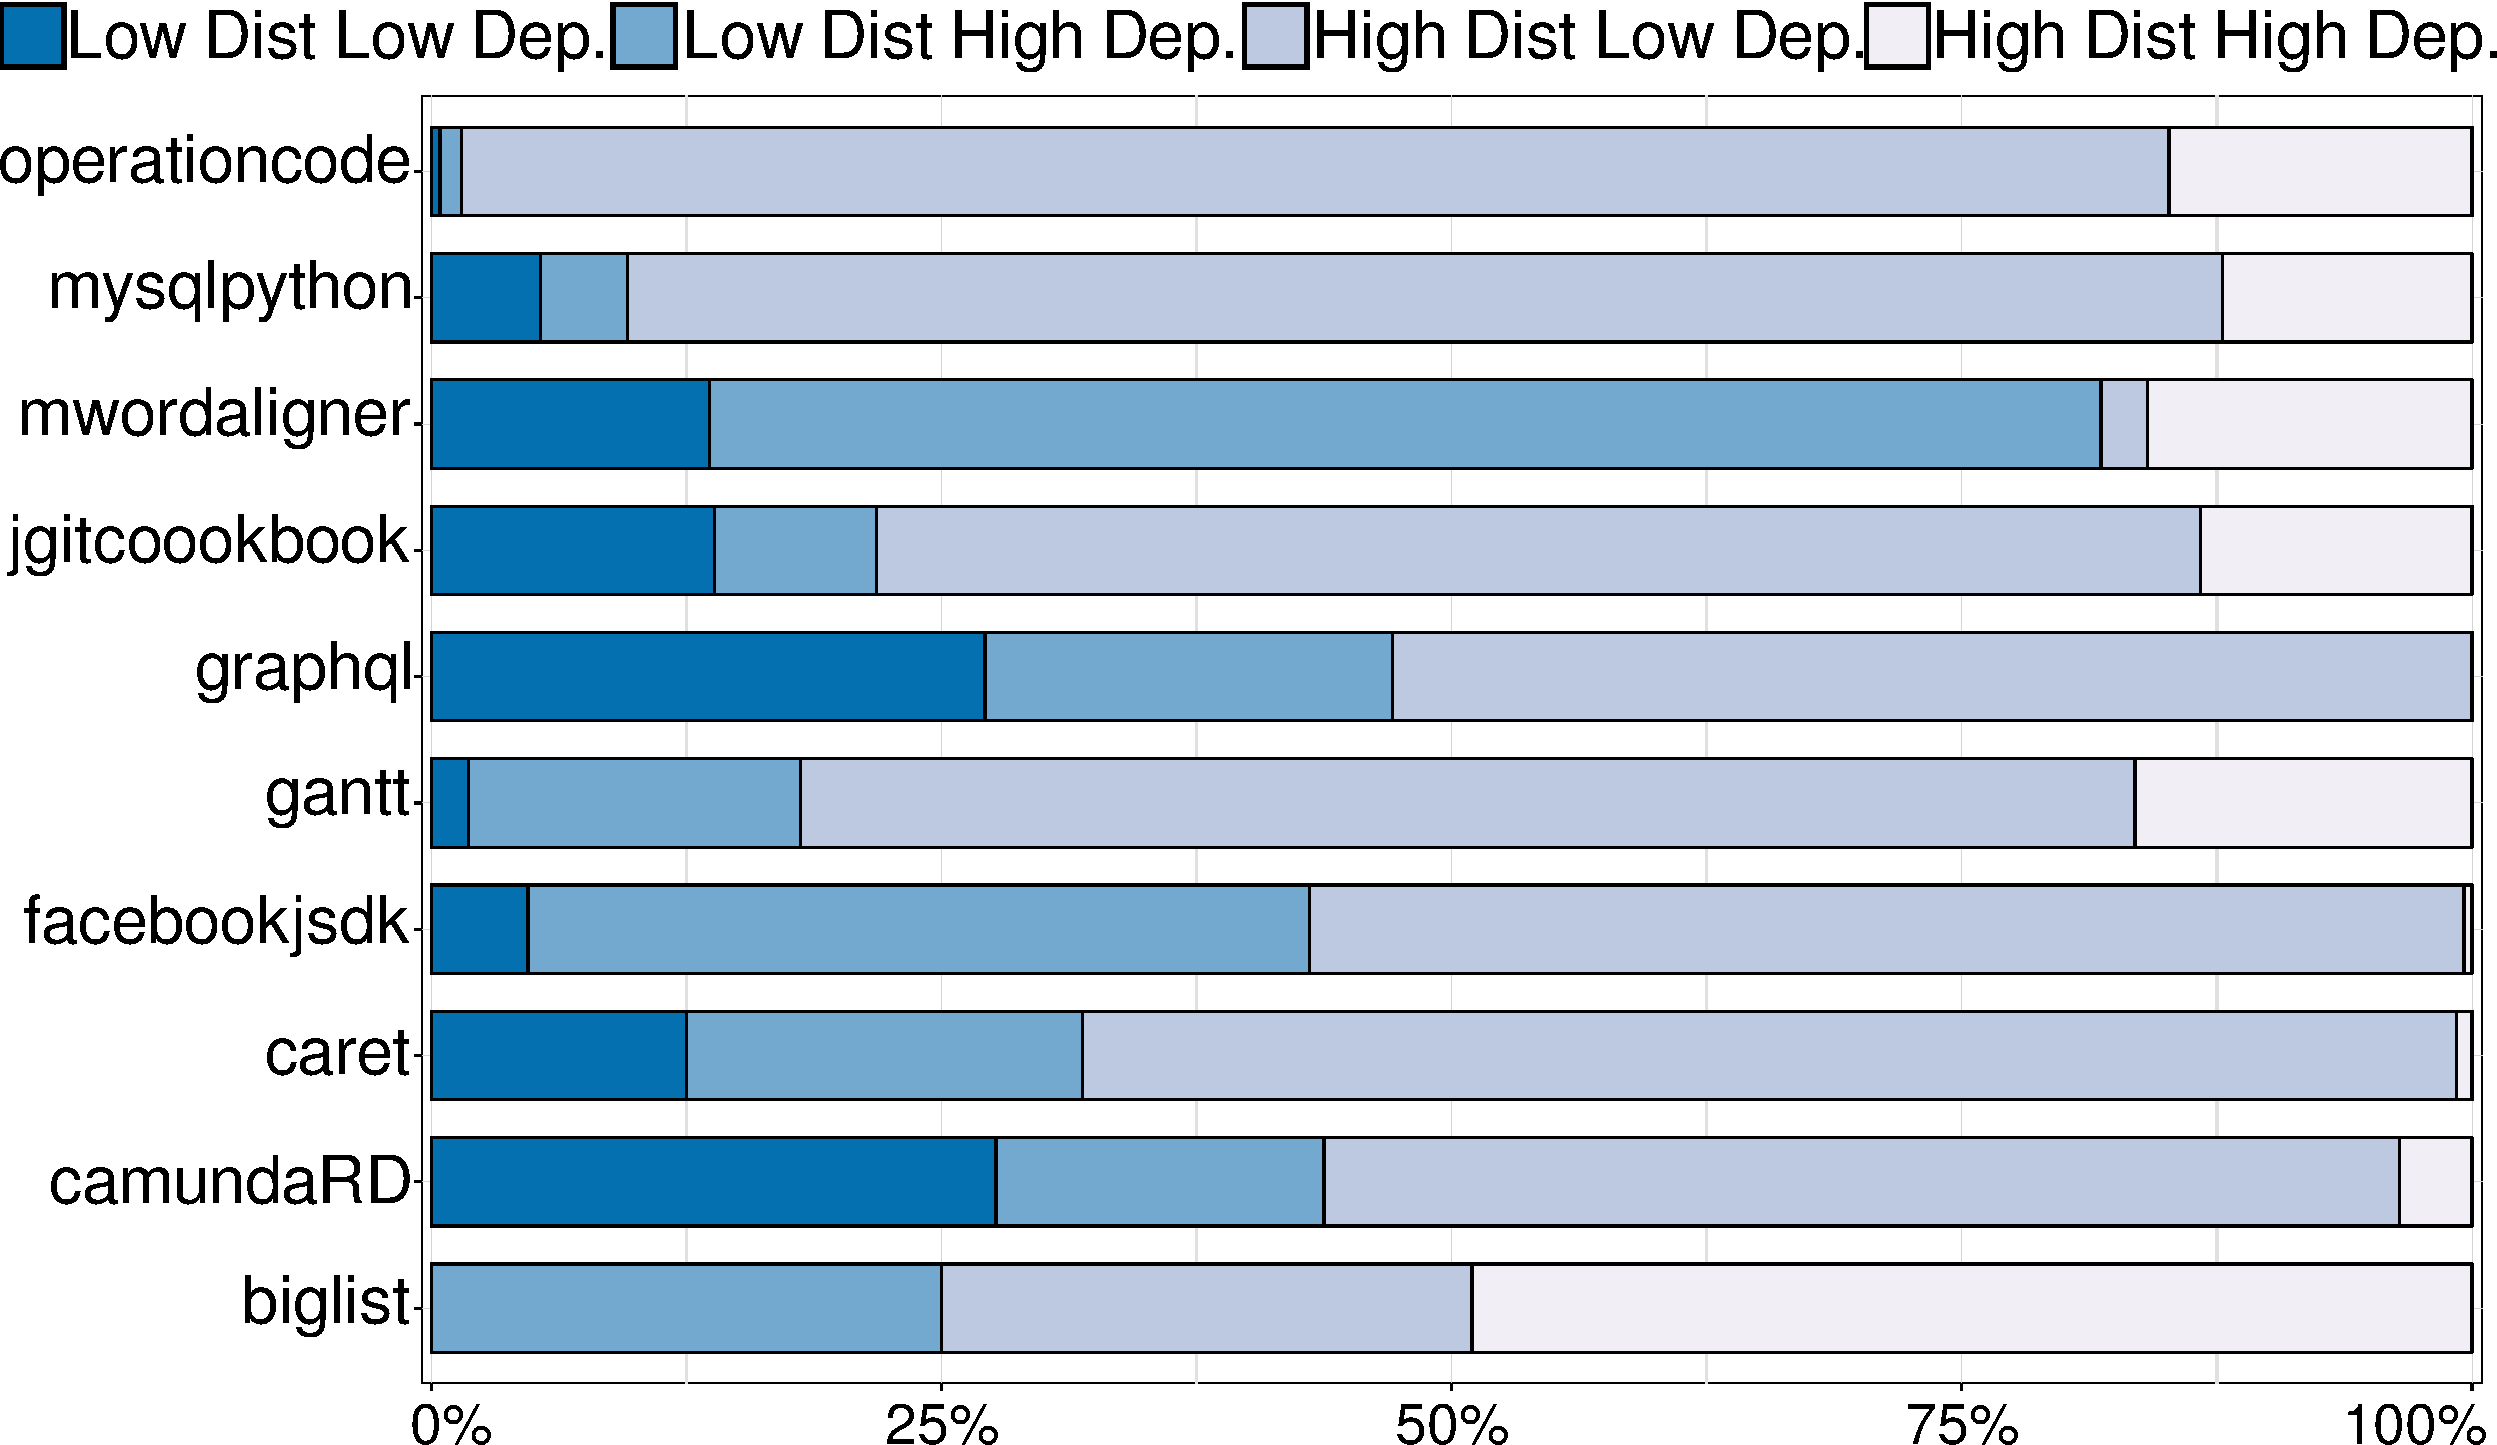
\includegraphics[width=.98\linewidth]{bpm2017/figures/Project-Analysis-Barchart-crop.pdf}
		\caption{Evaluation on real projects}
		\label{fig:project-analysis}
	\end{subfigure}~
	\begin{subfigure}[b]{.47\textwidth}
		\centering
		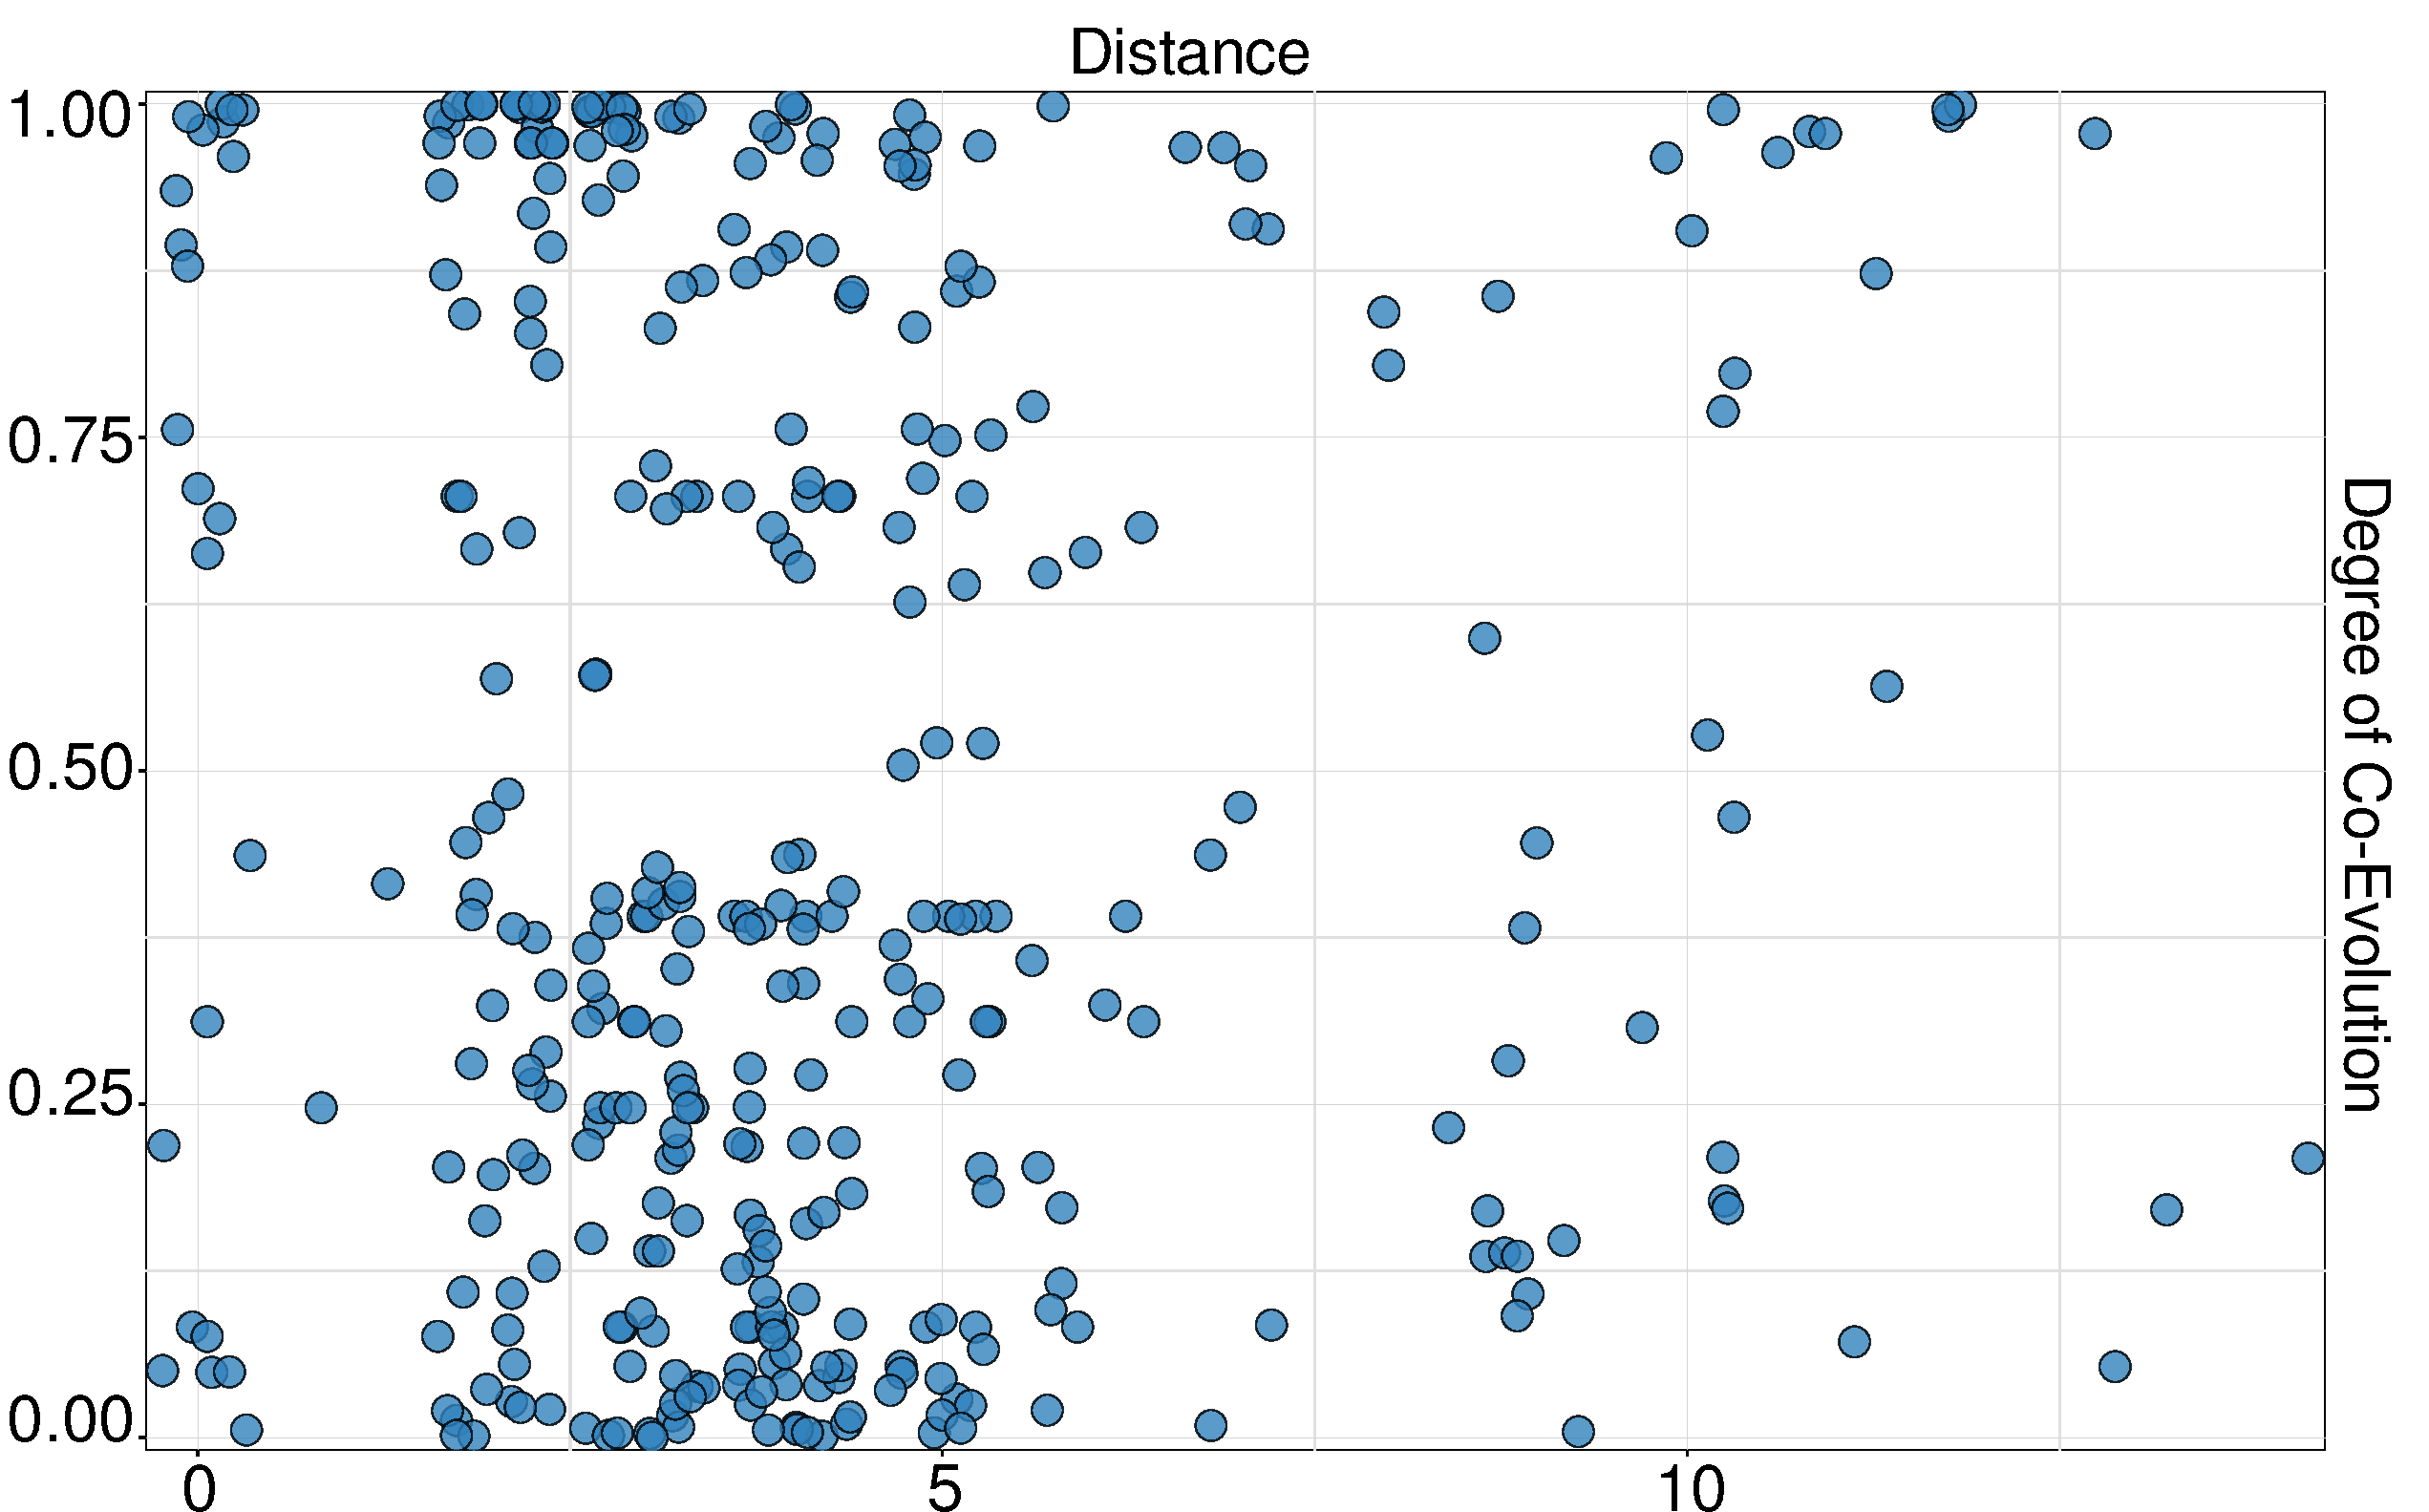
\includegraphics[width=.98\linewidth]{bpm2017/figures/Co-EvolutionVSDistance-OneColor.pdf}
		\caption{Distribution of pairs on real projects}
		\label{fig:pairs-on-space}
	\end{subfigure}
%	\vspace*{-.5cm}
	\caption{Characterization of the evaluated software projects}
\end{figure}
Next, we evaluate whether the work on files can be predicted. Zipf's law is typically used in corpus analysis and states that the \emph{frequency} of usage of any word is inversely proportional to its \emph{rank} in the frequency table. This approach has already been applied to software projects for understanding whether the assignment of developers to tasks in a software project could be predicted~\cite{Canfora2006}. Here, we focus on understanding whether the Zipf's law holds true also for work dependencies within a project. 

To this end, we selected one big and one small project from \Cref{table:evaluation-results-new}, namely \emph{Biglist} and \emph{Caret}. Biglist is a small project on a list of strings which are known to cause issues when used as user-input data. Caret is a big project consisting in the development of a sublime text editor for Chrome OS.
We collected how frequently were the artifacts worked on to generate a ranking. \Cref{fig:zipf-graph} depicts the corresponding charts and the fitted Zipf distribution. We notice that both projects present a similar distribution of values. This holds also for the other projects analyzed. In particular, Zipf's law is valid for the most frequently changed files. Afterwards, the distribution drops because of files not being worked anymore but still being part of the project.
%In pure software development projects, the tail can hint at some dead code and the need for maintenance.

\begin{figure}[t]
%	\centering
	\begin{subfigure}{.5\textwidth}
		\centering
		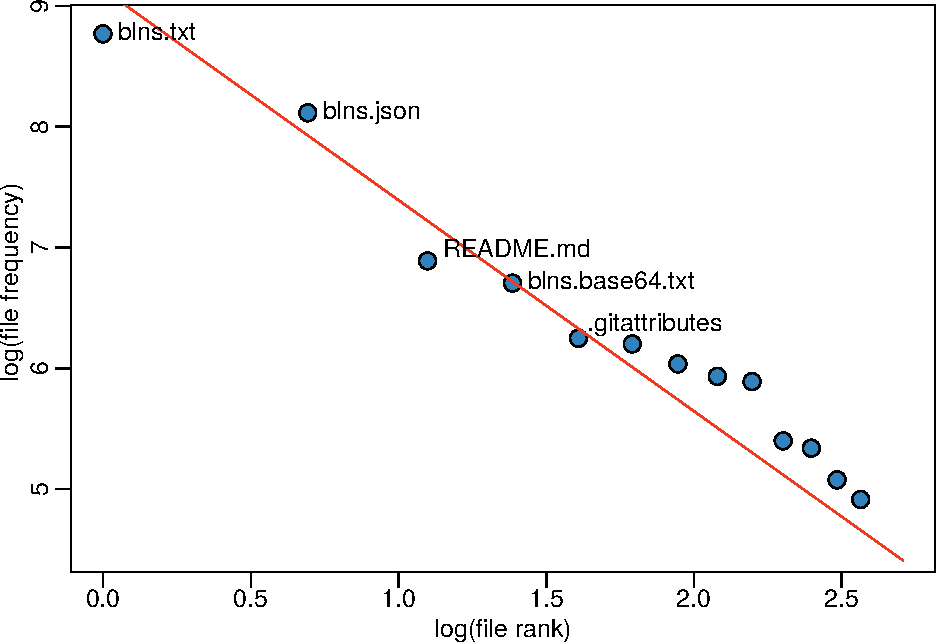
\includegraphics[width=\linewidth]{bpm2017/figures/biglist-new-crop}
		\caption{Biglist project}
		\label{fig:biglist}
	\end{subfigure}%
	\begin{subfigure}{.5\textwidth}
		\centering
		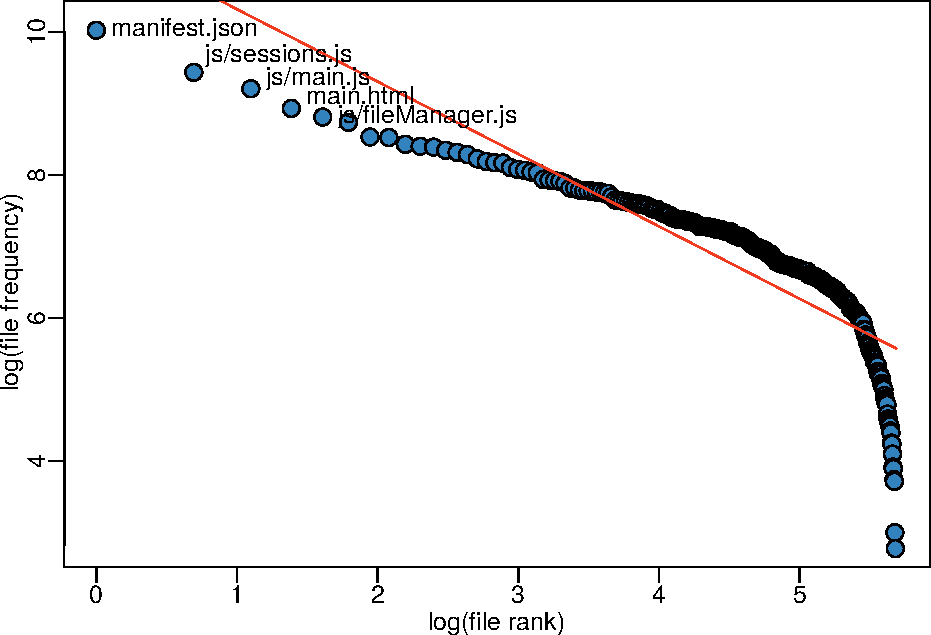
\includegraphics[width=\linewidth]{bpm2017/figures/caret-new-crop}
		\caption{Caret project}
		\label{fig:caret}
	\end{subfigure}
%	\vspace*{-.3cm}
	\caption{Zipf distribution of the worked files}
	\label{fig:zipf-graph}
\end{figure}
%\vspace*{-.2cm}

\section{Discussion}
\label{subsec:qualitative-eval}

In this section, we address requirement R1 by showing insights on the work history of files that are related. To this end we focused on the project \emph{smsr}, which has 21 commits over a time span of ten days.

%\todo[inline]{an example where it succeds:}
%\subsubsection{Example of work dependencies.}
%\subsubsection{Example of correct discovery.}
%\label{subsub:example}
Let us consider an example where our technique proves helpful. Our technique finds 6 highly related pairs, as shown in \Cref{table:evaluation-results-new}. We excluded files that have a functional dependencies, e.g. interface-class relations, where a change in the interface trivially brings change in the class. Thus, we were able to select the files \texttt{smsr/running example/Requirements/requirements.txt} and \texttt{smsr/running example/Software/model.java}, having $\chi=0.7$ and $d=4$. Moreover, by observing the content we verified that they do not have functional dependencies. Therefore, these two files are work dependent.
\Cref{fig:evaluated-processes} shows the extracted processes after mining their stories. Interestingly, the two processes do not share any activity because they were never changed together in the same commit.
%Literature approaches that leverage on network analysis can not uncover these type of dependencies, which are instead visible by the time series analysis.

\begin{figure}[t]
	\begin{subfigure}[t]{\textwidth}
		\centering
		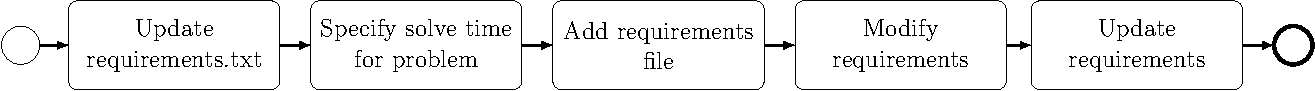
\includegraphics[width=.9\linewidth]{bpm2017/figures/six-processes/requirementsTxtProcess}
		\caption{Evolution of file \texttt{requirements.txt}}
		\label{subfig:requirements-file-process}
	\end{subfigure}
	\begin{subfigure}[ht]{\textwidth}
		\centering
		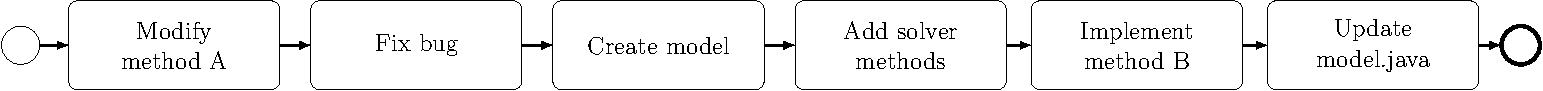
\includegraphics[width=.9\linewidth]{bpm2017/figures/six-processes/modelProcess.pdf}
		\caption{Evolution of file \texttt{model.java}}
		\label{subfig:model-file-process}
	\end{subfigure}
	\caption{Processes of two work-dependent files}
	\label{fig:evaluated-processes}
\end{figure}
%\todo[inline]{An example where it fails for some specific reason:}
%\subsubsection{Example of challenge.}

Our technique can fail under some circumstances. Consider the example above. We know that the files \texttt{requirements.txt} and \texttt{model.java} are work dependent. Let us now assume that the assumption of \emph{regular commits} in the \gls{vcs} does not hold. Nevertheless, we know that there is the following work pattern: \emph{at irregular times, one change in the requirements produces 2 changes of work that must be implemented in model in the next day}. In a short time window of 4 days, the time series would be $X_{req} = (1,0,1,0)$, $X_{model} = (0,2,0,2)$ and their correlation is $\sigma(f_{req},f_{model}) = -1$. Hence, they would score a high degree of co-evolution $\chi=1$. However, if we double the time window  and observe only another pattern the correlation would change. We get $X_{req} = (1,0,1,0,0,1,0,0)$, $X_{model} = (0,2,0,2,0,0,2,0)$ which score a $\sigma(f_{req},f_{model}) = -0.66$, $\chi=0.66$ and therefore not a high value of correlation.
%In these cases, approached that mine patterns of changes would outperform our approach.

These results show that our technique helps uncovering work dependencies that are not captured by existing approaches in literature which leverage on social network analysis~\cite{Zimmermann2008,Weicheng2013}. On the other hand, our technique is currently not yet able to retrieve dependencies with delay. We plan to address this challenge by using moving-average time series models. 

%\subsection{Discussion.}

\Cref{subsub:example} shows that time series analysis can help uncovering work dependencies that are not captured by existing approaches in literature which leverage on social network analysis~\cite{Zimmermann2008,Weicheng2013}. On the other hand, our technique is currently not yet able to retrieve dependencies with delay. We plan to address this challenge by using moving-average time series models.
%However, we argue that on the long run, under the assumption that \gls{vcs} is used in the everyday work, the technique can be useful to further 

